\chapter{Mijn lichaam}\label{ch:g1:my-body}

Ga voor een spiegel staan en zwaai: een heel levend lichaam zwaait
terug. Het groeit al van voor je geboorte, het buigt op sommige plekken
en op andere niet, en het is je hele leven van jou. Tijd om er zo naar
te kijken als we naar de kat en het madeliefje keken --- deel voor deel.

\section{De delen van mijn lichaam}

\begin{definition}[Delen van het menselijk lichaam]\label{def:g1:my-body:parts}
Het menselijk lichaam heeft drie hoofddelen:
\begin{enumerate}
  \item het \emph{hoofd}\index{hoofd}, dat het gezicht, de ogen, de
        oren, de neus en de mond draagt;
  \item de \emph{romp}\index{romp}, het middenstuk van het lichaam ---
        borst, buik en rug;
  \item de \emph{ledematen}\index{ledemaat}: twee \emph{armen}\index{arm}
        die in handen eindigen, twee \emph{benen}\index{been} die in voeten eindigen.
\end{enumerate}
Het hoofd rust op de \emph{hals}\index{hals}, die het met de romp
verbindt.
\end{definition}

\begin{omfigure}
\begin{tikzpicture}
  \node[anchor=south west, inner sep=0] (img) at (0,0)
    {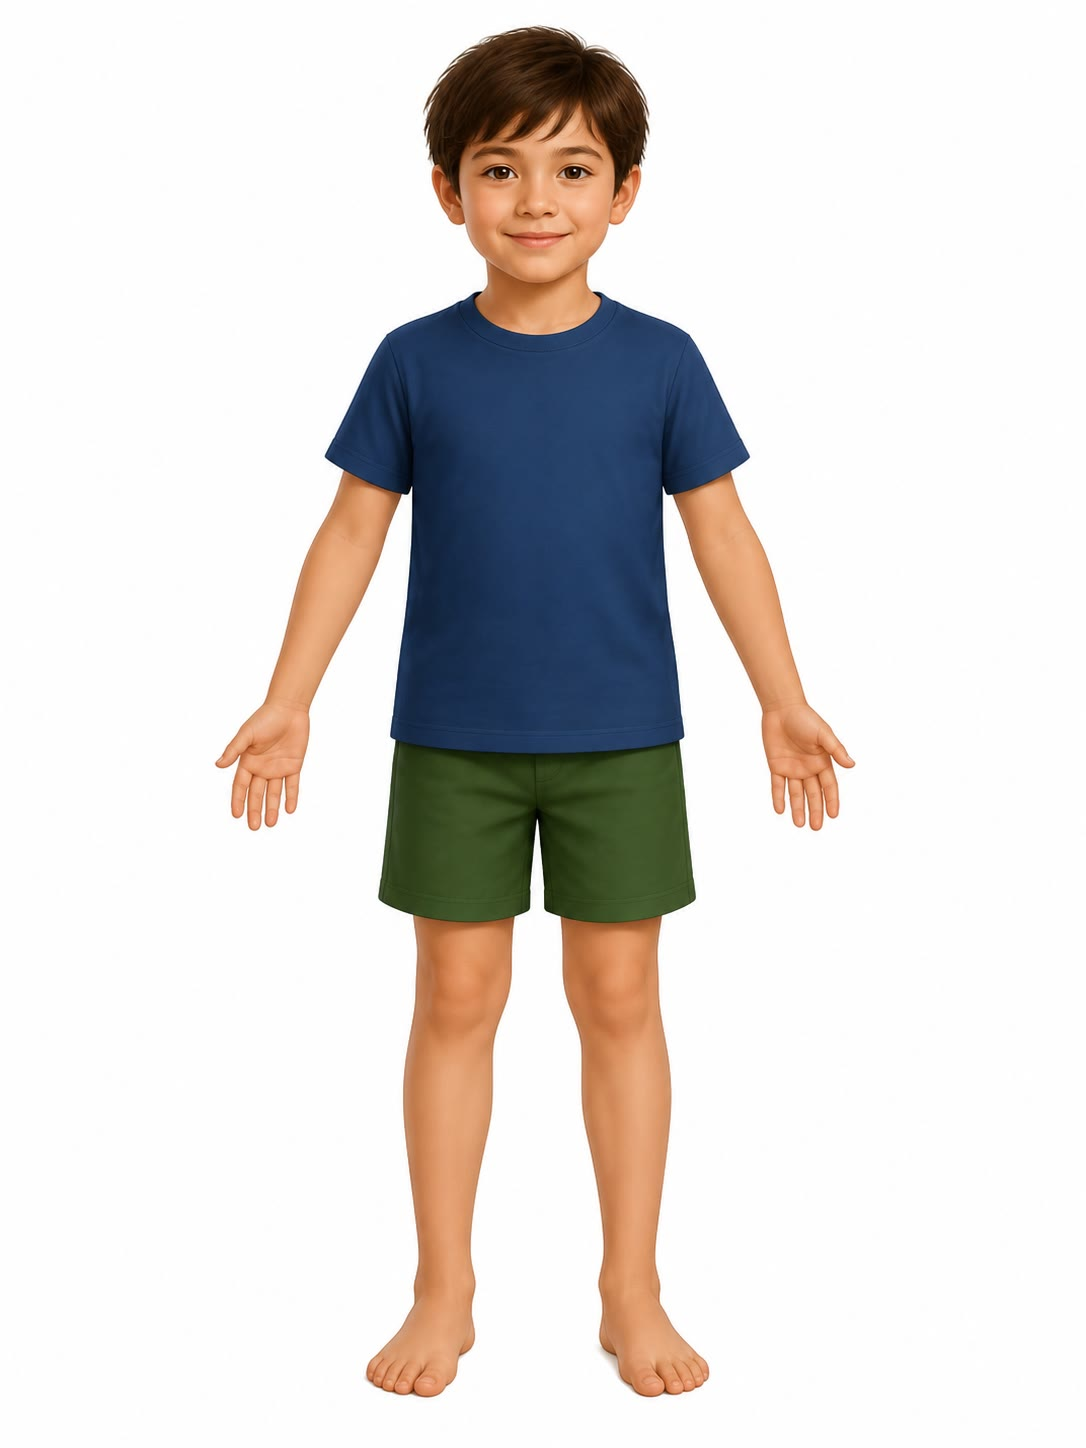
\includegraphics[width=0.42\linewidth]{images/book1/ai/fig-child-standing.jpg}};
  \begin{scope}[x={(img.south east)}, y={(img.north west)},
      every node/.style={font=\small}]
    \draw[omDef, thick] (0.57,0.90) -- (0.76,0.92) node[right] {hoofd};
    \draw[omDef, thick] (0.53,0.80) -- (0.76,0.83) node[right] {hals};
    \draw[omDef, thick] (0.58,0.62) -- (0.78,0.66) node[right] {romp};
    \draw[omDef, thick] (0.74,0.46) -- (0.86,0.38)
      node[below, align=center] {arm en\\ hand};
    \draw[omDef, thick] (0.60,0.18) -- (0.78,0.14)
      node[right, align=left] {been en\\ voet};
  \end{scope}
\end{tikzpicture}

{\small De drie hoofddelen van het lichaam: \omterm{def:g1:my-body:parts}{hoofd}, \omterm{def:g1:my-body:parts}{romp} en vier
\omterm{def:g1:my-body:parts}{ledematen} --- met de \omterm{def:g1:my-body:parts}{hals} die \omterm{def:g1:my-body:parts}{hoofd} en \omterm{def:g1:my-body:parts}{romp} verbindt.}
\end{omfigure}

\begin{example}[Hetzelfde plan als de kat?]\label{ex:g1:my-body:cat}
Vergelijk jezelf met de kat: kop, \omterm{def:g1:my-body:parts}{romp}, vier \omterm{def:g1:my-body:parts}{ledematen} --- het plan
lijkt op elkaar. Maar de kat loopt op alle vier; jij staat op twee
\omterm{def:g1:my-body:parts}{benen} en houdt twee \omterm{def:g1:my-body:parts}{armen} vrij om te dragen, te tekenen en te zwaaien.
En waar de kat een \omterm{def:g1:animals-around-us:parts}{staart} heeft, heb jij er geen.
\end{example}

\section{Buigen: de gewrichten}

\begin{definition}[Gewricht]\label{def:g1:my-body:joint}
Een \emph{gewricht}\index{gewricht} is een plaats waar het lichaam kan
buigen of draaien. De \emph{elleboog}\index{elleboog} buigt de \omterm{def:g1:my-body:parts}{arm}, de
\emph{knie}\index{knie} buigt het \omterm{def:g1:my-body:parts}{been}, de
\emph{schouder}\index{schouder} draait de hele \omterm{def:g1:my-body:parts}{arm}, de
\emph{pols}\index{pols} en de \emph{enkel}\index{enkel} buigen de hand
en de voet. Tussen twee gewrichten blijft het lichaam recht.
\end{definition}

\begin{omfigure}
\begin{tikzpicture}[scale=1.0]
  % straight arm
  \draw[very thick] (0,0) -- (2.0,0);
  \draw[very thick] (2.0,0) -- (3.8,0);
  \fill[omThm] (2.0,0) circle (0.1);
  \fill[omDef!60] (0,0) circle (0.1);
  \draw[thick, fill=omDef!8] (4.0,0) circle (0.18);
  \node[below, font=\small] at (1.9,-0.3) {arm recht gehouden};
  % bent arm
  \begin{scope}[xshift=6.6cm]
    \draw[very thick] (0,0) -- (2.0,0);
    \draw[very thick] (2.0,0) -- (3.1,1.45);
    \fill[omThm] (2.0,0) circle (0.1);
    \fill[omDef!60] (0,0) circle (0.1);
    \draw[thick, fill=omDef!8] (3.22,1.6) circle (0.18);
    \node[below, font=\small] at (1.9,-0.3) {arm gebogen in de elleboog};
    \draw[omThm] (2.05,0.12) -- (1.55,0.8)
      node[above left, font=\small, omThm] {het gewricht buigt};
  \end{scope}
  \node[font=\small] at (1.0,1.4) {schouder};
  \draw[omDef!60] (0.05,0.12) -- (0.55,1.15);
\end{tikzpicture}

{\small De \omterm{def:g1:my-body:parts}{arm} buigt alleen in zijn \omterm{def:g1:my-body:joint}{gewrichten}: \omterm{def:g1:my-body:joint}{schouder} (blauw) en
\omterm{def:g1:my-body:joint}{elleboog} (rood). Daartussen blijft hij recht.}
\end{omfigure}

\begin{example}[Probeer het: lopen met stijve knieën]\label{ex:g1:my-body:stiff}
Probeer eens te lopen zonder je knieën te buigen. Het lukt --- maar net
--- met stijve kleine eendenpasjes. Probeer nu een potlood van de vloer
te rapen zonder knieën, heupen of rug te buigen. \omterm{def:g1:my-body:joint}{Gewrichten} maken de
bewegingen van het lichaam soepel, snel en gemakkelijk.
\end{example}

\begin{remark}[Rechts en links]\label{rem:g1:my-body:sides}
Het lichaam heeft twee kanten, rechts en links, bijna als een spiegel:
aan elke kant een \omterm{def:g1:my-body:parts}{arm} en een \omterm{def:g1:my-body:parts}{been}, aan elke kant van het \omterm{def:g1:my-body:parts}{hoofd} een oog
en een oor. Je rechterhand van je linkerhand kunnen onderscheiden is
ook lichaamskennis --- het vertelt anderen welke kant je bedoelt.
\end{remark}

\section{Mijn lichaam groeit}

\begin{proposition}[Opgroeien]\label{prop:g1:my-body:growth}
Het lichaam van een kind \emph{groeit}\index{groeien}: het wordt jaar
na jaar langer en zwaarder, tot het volwassen is. Groeien gaat langzaam
en gestaag --- te langzaam om te voelen, gemakkelijk om te meten.
\end{proposition}
\admitted

\begin{example}[Streepjes op de deurpost]\label{ex:g1:my-body:doorframe}
Ga tegen de deurpost staan; een volwassene zet met een potlood een
streepje bij je lengte. Doe het een paar maanden later nog eens: het
nieuwe streepje staat hoger! Je hebt jezelf nooit voelen groeien, maar
de twee streepjes, het ene boven het andere, laten het duidelijk zien.
\end{example}

\begin{omfigure}
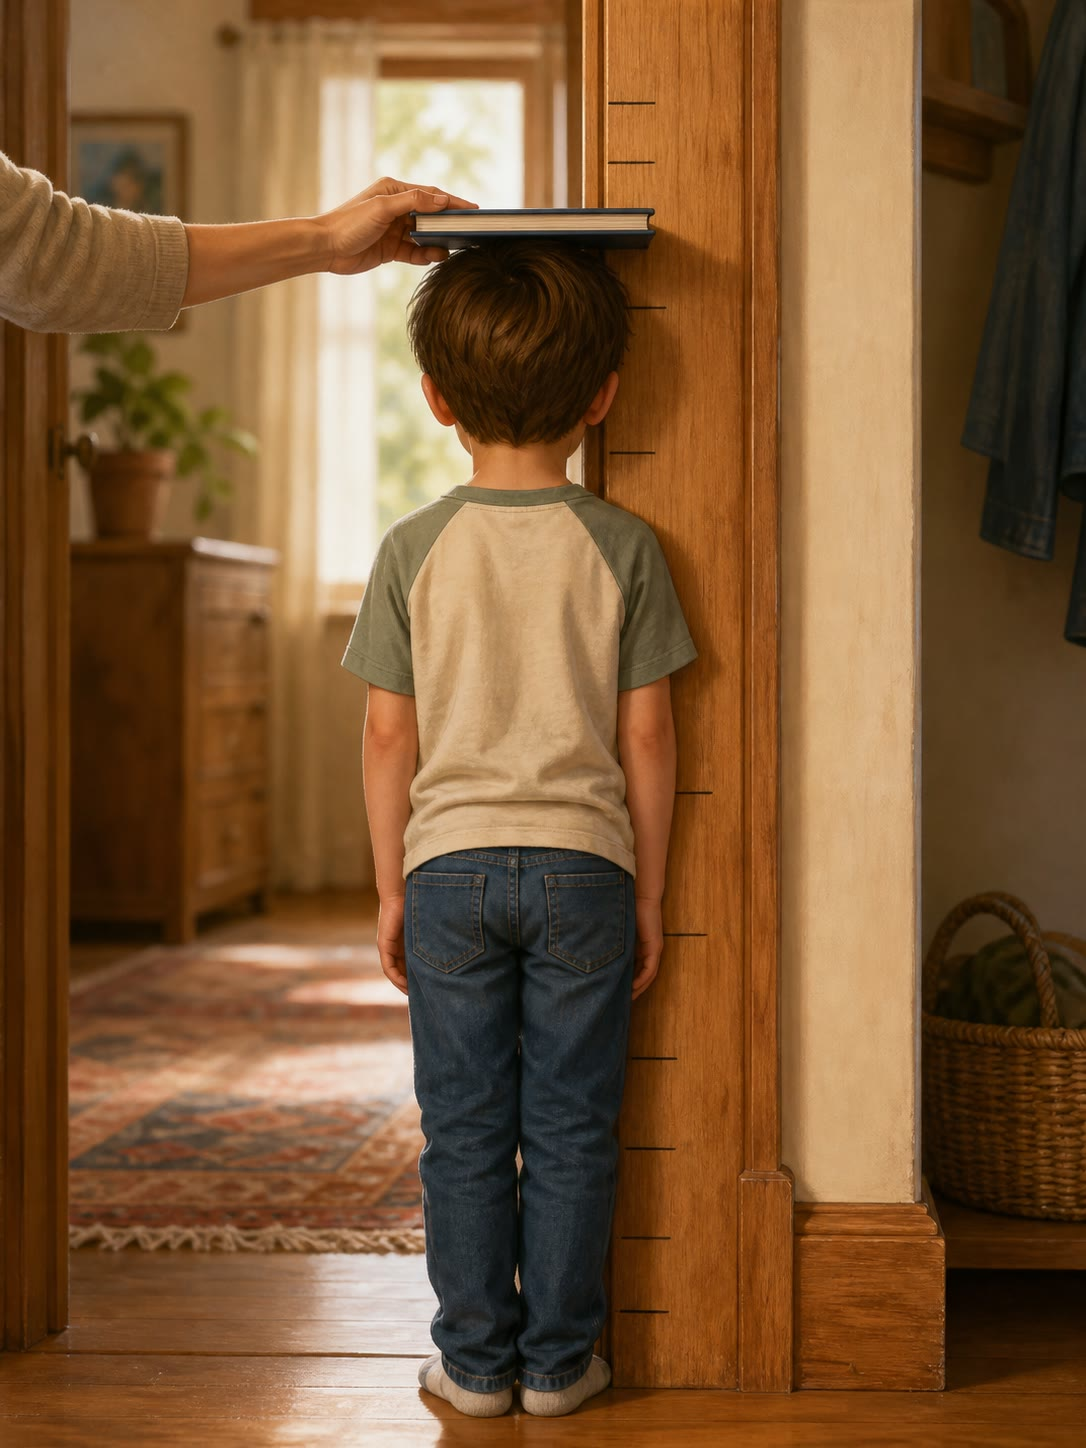
\includegraphics[width=0.46\linewidth]{images/book1/ai/g1-body-doorframe.jpg}

{\small Meetdag bij de deurpost: het platte boek brengt de bovenkant
van het \omterm{def:g1:my-body:parts}{hoofd} recht naar het hout.}
\end{omfigure}

\begin{method}[Mijn lengte meten]\label{met:g1:my-body:measure}
\begin{enumerate}
  \item Doe je schoenen uit;
  \item ga recht staan, met rug en hielen tegen de muur en je blik
        vooruit;
  \item een helper legt een plat boek waterpas op je \omterm{def:g1:my-body:parts}{hoofd}, tegen de
        muur aan;
  \item zet een streepje onder het boek, en schrijf de datum ernaast.
\end{enumerate}
Als je elke keer op dezelfde manier meet, kun je de streepjes
vertrouwen --- en vergelijken.
\end{method}

\begin{remark}[Elk lichaam is anders]\label{rem:g1:my-body:different}
In één klas zijn sommige kinderen langer, andere kleiner; sommige
groeien vroeger, andere later. Dat is allemaal normaal. Lichamen zijn
als gezichten: op hetzelfde plan gebouwd, en elk anders. De streepjes
op jouw deurpost zijn van jou --- ze zijn er niet om met de buren te wedijveren.
\end{remark}

\section{Oefeningen}

\begin{exercise}[$\star$]\label{exo:g1:my-body:1}
Noem de drie hoofddelen van het menselijk lichaam. Wat verbindt het
\omterm{def:g1:my-body:parts}{hoofd} met de \omterm{def:g1:my-body:parts}{romp}?
\end{exercise}

\begin{exercise}[$\star$]\label{exo:g1:my-body:2}
Waarin eindigt elk \omterm{def:g1:my-body:parts}{ledemaat} --- wat zit er aan het eind van een \omterm{def:g1:my-body:parts}{arm}, en
aan het eind van een \omterm{def:g1:my-body:parts}{been}?
\end{exercise}

\begin{exercise}[$\star$]\label{exo:g1:my-body:3}
Welk \omterm{def:g1:my-body:joint}{gewricht} buigt: (a) de \omterm{def:g1:my-body:parts}{arm} in het midden? (b) het \omterm{def:g1:my-body:parts}{been} in het
midden? (c) de hand aan het eind van de \omterm{def:g1:my-body:parts}{arm}?
\end{exercise}

\begin{exercise}[$\star$]\label{exo:g1:my-body:4}
Raak je rechteroor aan met je linkerhand. Welke \omterm{def:g1:my-body:joint}{gewrichten} heeft je \omterm{def:g1:my-body:parts}{arm}
zojuist gebruikt? Noem er minstens twee.
\end{exercise}

\begin{exercise}[$\star$]\label{exo:g1:my-body:5}
Zoek in \cref{ex:g1:my-body:cat} één manier waarop jouw lichaam op dat
van de kat lijkt en twee manieren waarop het verschilt.
\end{exercise}

\begin{exercise}[$\star$]\label{exo:g1:my-body:6}
Waarom legt de helper in \cref{met:g1:my-body:measure} een plat boek op
je \omterm{def:g1:my-body:parts}{hoofd} in plaats van alleen maar te kijken?
\end{exercise}

\begin{exercise}[$\star$]\label{exo:g1:my-body:7}
Twee streepjes op de deurpost: dat van vorig jaar, en dat van vandaag
iets hoger. Wat laten de streepjes zien? Heb je het voelen gebeuren?
\end{exercise}

\begin{exercise}[$\star$]\label{exo:g1:my-body:8}
Probeer het: loop met stijve knieën zoals in \cref{ex:g1:my-body:stiff},
en probeer daarna te klappen zonder je ellebogen te buigen. Welke
alledaagse bewegingen blijken \omterm{def:g1:my-body:joint}{gewrichten} nodig te hebben?
\end{exercise}

\begin{exercise}[$\star\star$]\label{exo:g1:my-body:9}
Mia is de kleinste van haar klas en maakt zich daar zorgen over. Wat
antwoordt \cref{rem:g1:my-body:different} haar?
\end{exercise}

\begin{exercise}[$\star\star$]\label{exo:g1:my-body:10}
Een pop van één houten stok kan niet op een stoel zitten. Waar zou jij
de stok doorsnijden en draaipunten toevoegen zodat hij kan zitten? Noem
de lichaamsgewrichten die jouw sneden nabootsen.
\end{exercise}
